\section{Modeling Pine Island Glacier}
\subsection{Goals} %{{{
\begin{itemize}
	\item Model Pine Island Glacier
	\item Follow an example of how to create a mesh and set up the floating ice shelf of a real-world glacier
	\item Use observational data to parameterize the model
	\item Learn how to use inversions to infer basal friction and plot the results
\end{itemize}
%}}}
\subsection{Introduction}%{{{
In this example, the main goal is to parameterize and model a real glacier. In order to build an operational simulation of Pine Island Glacier, we will follow these steps:
\begin{itemize}
	\item Define the model region
	\item Create a mesh
	\item Apply masks
	\item Parameterize the model
	\item Invert friction coefficient
	\item Plot results
	\item Run higher-order simulation
\end{itemize}

Files needed for this tutorial can be found in \verb@trunk/examples/Pig/@. The \verb@runme.m@ file contains the structure of the simulation, while the \verb@.par@ file includes most parameters needed for the model set-up. The \verb@.exp@ files are shape files that define geometric boundaries of the simulation.

Observed datasets needed for the parameterization also need to be \href{https://issm.jpl.nasa.gov/documentation/tutorials/datasets/}{downloaded}.
%}}}
\subsection{Setting-up domain outline} %{{{
We first draw the domain outline of Pine Island Glacier based on observed velocity map. First, run \verb@PigRegion.m@ in MATLAB. It produces a figure with the observed velocities:
\begin{figure}[H]
	\begin{center}
		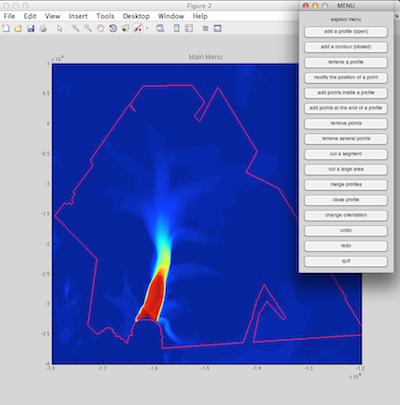
\includegraphics[scale=0.9]{/assets/img/using-issm/tutorials/pig/exptool.png}
	\end{center}
\end{figure}

You can then use the \verb@exptool@ to draw the model domain:
\begin{verbatim}>> exptool('PigDomain.exp')\end{verbatim}

NOTE: if you have not \href{https://issm.jpl.nasa.gov/documentation/tutorials/datasets/}{downloaded the datasets}, you will get the following error:
\begin{verbatim}Could not open ../Data/Antarctica_ice_velocity.nc."\end{verbatim}
If this occurs, go into the \verb@Data@ directory and run the script to download the datasets. You
will not be able to proceed until you do so.

This example shows you how to create your own model boundary, but for the rest of the tutorial, we
will be using the provided domain outline, which is \verb@ModelDomain.bkp@. Rename this file \verb@ModelDomain.exp@ (which will, effectively, erase your contour):
\begin{verbatim}>>!mv DomainOutline.bkp DomainOutline.exp\end{verbatim}
%}}}
\subsection{Mesh}%{{{
The first step is to create the mesh of the model domain.

In the \verb@runme.m@ file, the mesh is generated in a multi-step process. Open the \verb@runme.m@ file and make sure that the variable \verb@steps@, at the top of the file, is set to \verb@steps=[1]@. In the code, you will see that in step 1 the following actions are implemented:

\begin{itemize}
	\item a uniform mesh is created
	\item the mesh is then refined using anisotropic mesh refinement. We use the surface velocity as a metric
	\item Set the mesh parameters
	\item Plot the model and load the velocities from \verb@http://nsidc.org/data/nsidc-0484.html@
	\item Get the necessary data to build up the velocity grid
	\item Get velocities (note: You can use \verb@ncdisp('file')@ to see an \verb@ncdump@)
	\item Interpolate the velocities onto a coarse mesh. Adapt the mesh to minimize error in velocity interpolation
	\item Plot the mesh
	\item Save the model
\end{itemize}

Execute the \verb@runme.m@ file to perform step 1. You should see the following figure:
\begin{figure}[H]
	\begin{center}
	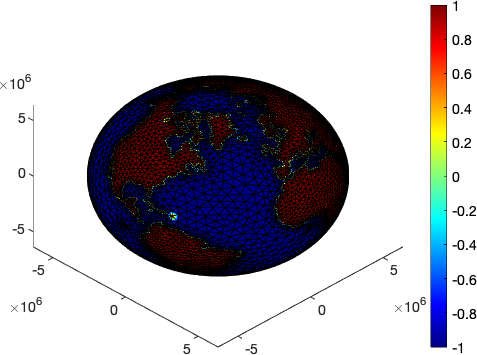
\includegraphics[scale=1.0]{/assets/img/using-issm/tutorials/pig/Mesh.png}
	\end{center}
\end{figure}
%}}}
\subsection{Mask}%{{{
The second step of the \verb@runme.m@ creates the masks required to specify where there is ice in the domain, and where the ice is grounded.

First, we specify where the ice is grounded and floating in the domain:
\begin{itemize}
	\item The field \verb@md.mask.ocean_levelset@ contains this information
		\begin{itemize}
			\item Ice is grounded if \verb@md.mask.ocean_levelset@ is positive
			\item Ice is floating if \verb@md.mask.ocean_levelset@ is negative
			\item The grounding line lies where \verb@md.mask.ocean_levelset@ equals zero
		\end{itemize}
\end{itemize}

Then we specify where ice is present:
\begin{itemize}
	\item The field \verb@md.mask.ice_levelset@ contains this information
		\begin{itemize}
			\item Ice is present if \verb@md.mask.ice_levelset@ is negative
			\item There is no ice if \verb@md.mask.ice_levelset@ is positive
			\item The ice front lies where \verb@md.mask.ice_levelset@ equals zero
		\end{itemize}
\end{itemize}

Open \verb@runme.m@ and set \verb@steps=[2]@. Now, execute the \verb@runme.m@ file to run step 2.

After executing step 2, you should see the following figure that represents the mask:
\begin{figure}[H]
	\begin{center}
		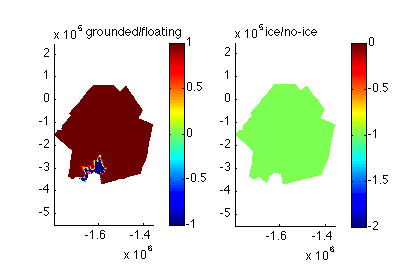
\includegraphics[scale=1.1]{/assets/img/using-issm/tutorials/pig/Mask2.png}
	\end{center}
\end{figure}
%}}}
\subsection{Parameterization}%{{{
Parameterization of models is usually done through a different file (\verb@Pig.par@). Parameters which are unlikely to change for a given set of experiments are set there to lighten the \verb@runme.m@ file. In this example we use SeaRISE data to parameterize the following model fields:

\begin{itemize}
	\item Geometry
	\item Initialization parameters
	\item Material parameters
	\item Forcings
	\item Friction coefficient
	\item Boundary conditions
\end{itemize}

Some parameters are adjusted in \verb@runme.m@, as they are likely to be changed during the simulation. This is the case for the stress balance equation that is set-up using \verb@setflowequation@

Now, change the \verb@runme.m@ file as before, and run step 3 to perform the Parameterization.
%}}}
\subsection{Inversion of basal friction}%{{{
The friction coefficient is inferred from the surface velocity using the following friction law:
\begin{equation}
	\mathbf{ \tau }_b = -\beta^{2} N^r \|\mathbf{v_b}\|^{s-1}\mathbf{v_b}
\end{equation}

\begin{itemize}
	\item $\mathbf{ \tau }_b$ : Basal drag
	\item $N$: Effective pressure
	\item $v_b$: Basal velocity (equal surface in SSA approximation)
	\item $r$: Exponent (equals $q/p$ of the parameter file)
	\item $s$: Exponent (equals $1/p$ of the parameter file)
\end{itemize}

The procedure for the inversion is as follows:
\begin{itemize}
	\item Velocity is computed from the SSA approximation
	\item Misfit of the cost function is computed
	\item Friction coefficient is modified following the gradient of the cost function
\end{itemize}

All the parameters that can be adjusted for the inversion are in \verb@md.inversion@.

Run step 4 and look at the results, they should be similar to the figure below:
\begin{figure}[H]
	\begin{center}
		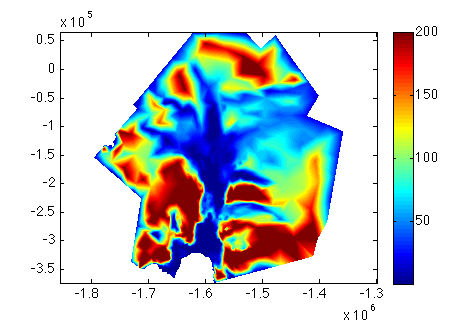
\includegraphics[scale=1.0]{/assets/img/using-issm/tutorials/pig/ControlMethod.png}
	\end{center}
\end{figure}
%}}}
\subsection{Plot results}%{{{
Plotting ability are mainly based on \verb@plotmodel@ for simple graphs. However, you can also use or create your own routines.

Change the step to 5 and run the simulation. It should create the following figure:
\begin{figure}[H]
	\begin{center}
		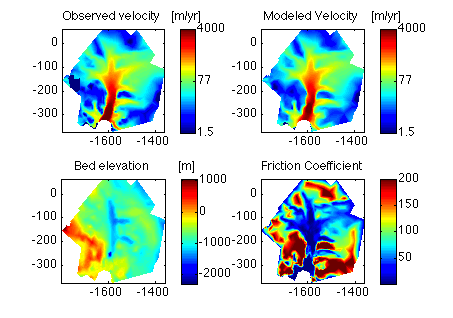
\includegraphics[scale=1.2]{/assets/img/using-issm/tutorials/pig/Plot.png}
	\end{center}
\end{figure}
%}}}
\subsection{Higher Order (HO) Ice Flow Model}%{{{
The last step of this tutorial is to run a forward model of Pine Island Glacier with the Higher-Order stress balance approximation.

The following steps need to be performed in \verb@step 7@ of the \verb@runme.m@ file:
\begin{itemize}
	\item Load the previous step
		\begin{itemize}
			\item Model to load is \verb@Control_drag@
		\end{itemize}
	\item Disable the inversion process
		\begin{itemize}
			\item Change \verb@iscontrol@ to zero the inversion flag (\verb@md.inversion@)
		\end{itemize}
	\item Extrude the mesh
		\begin{itemize}
			\item \verb@help extrude@
			\item Keep the number of layers low to avoid long computational time
		\end{itemize}
	\item Change the stress balance approximation
		\begin{itemize}
			\item Use the function \verb@setflowequation@
		\end{itemize}
	\item Solve
		\begin{itemize}
			\item We are still solving for a \verb@StressBalanceSolution@
		\end{itemize}
	\item Save the model as in the preceding steps
\end{itemize}

If you need help, the solution is provided below.

Step 7 provides a comparison of the Shelfy-Stream and Higher-Order approximations. The following figure should be created if you run step 7:
\begin{figure}[H]
	\begin{center}
		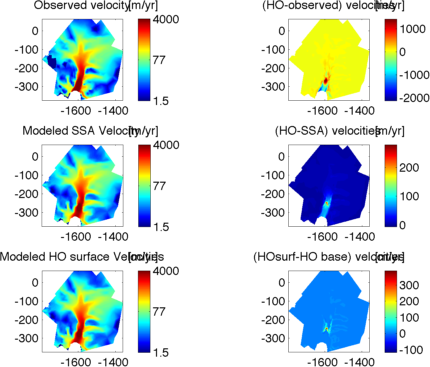
\includegraphics[scale=1.2]{/assets/img/using-issm/tutorials/pig/VelocityComparison.png}
	\end{center}
\end{figure}
%}}}
\subsection{Solution for step 6}%{{{
\begin{verbatim}if any(steps==6)
	md = loadmodel('./Models/PIG_Control_drag');
	md.inversion.iscontrol=0;

	disp('   Extruding mesh')
	number_of_layers=3;
	md=extrude(md,number_of_layers,1);

	disp('   Using HO Ice Flow Model')
	md=setflowequation(md, 'HO', 'all');

	md=solve(md,'Stressbalance');

	save ./Models/PIG_ModelHO md;
end\end{verbatim}
